%%%%%%%%%%%%%%%%%%%%%%%%%%%%%%%%%%%%%%%%%%%%%%%%%%%%%%%%%%
%                                                                                      %
%         Univesity College London Project LaTex Template            %
%                                                                                      %
%%%%%%%%%%%%%%%%%%%%%%%%%%%%%%%%%%%%%%%%%%%%%%%%%%%%%%%%%%
%
%   Author: Alex Charles           Email: aep.charles@gmail.com
%
% -----------------------------------------------------------------------------------
%      PACKAGES & OTHER DOCUMENT CONFIGURATIONS
% -----------------------------------------------------------------------------------
\documentclass[fontsize=10pt]{extarticle}

\usepackage[utf8]{inputenc}
\usepackage[T1]{fontenc}
\usepackage[british]{babel}
% ----------NEW BIBLATEX BIBLIOGRAPHY-----------------------------------------------
\usepackage[eprint=false,backend=bibtex,style = ieee]{biblatex} % Upgrades Bibliography Block Ragged helps break lines in url fixes error

\addbibresource{BibFile.bib} %%% For biblatex
%e.g to add page number \footfullcite[chapter, p.~215]{AAIB}
% This allows can use footfullcite commands
% Note urldate field must be in yyyy-mm-dd to work - use online type
% Remeber to use \printbibliography in the footer
% -----------------------------------------------------------------------------------
% \usepackage{sectsty}
\usepackage{url}

%%% --- The following two lines are what needs to be added --- %%%
\setcounter{biburllcpenalty}{7000}
\setcounter{biburlucpenalty}{8000}

\usepackage{amssymb,amsmath}
\numberwithin{figure}{section} %%%%% <<<<<< Puts Figure Numbering into Sections
\usepackage{ifxetex,ifluatex}  %<<<<<<<<< Edit FONT HERE
\ifnum 0\ifxetex 1\fi\ifluatex 1\fi=0 % if pdftex
  \usepackage[T1]{fontenc}
  \usepackage[utf8]{inputenc}
\else % if luatex or xelatex
  \ifxetex
    \usepackage{mathspec}
    \setmainfont[
 BoldFont={AvenirNext-Medium},ItalicFont={AvenirNext-Italic},
 BoldItalicFont={AvenirNext-MediumItalic}]{AvenirNext-Regular}
  \else
  % Font Package for XeLatex
    \usepackage{fontspec}
    \setmainfont{AvenirNext-Regular}
  \fi
  \defaultfontfeatures{Ligatures=TeX,Scale=MatchLowercase}
\fi
\usepackage[fit]{truncate} %Truncates headers that are too long
\usepackage[headheight=26pt,headsep=0.15cm]{geometry}
\usepackage{fancyhdr}
\usepackage{lastpage}
\usepackage{extramarks}
\usepackage{gensymb}
\usepackage{lipsum}
\usepackage{float}
\usepackage{graphicx}
\graphicspath{{TempImg/}{Img/}}%<<<<<<<<< Location of Template Images and Other Images, Add folders here
\usepackage{subfig}
\usepackage{wrapfig}
\usepackage[font ={small,it}]{caption}
\usepackage{amsfonts,amsthm} % Math packages
% \usepackage{cite}
\usepackage{csquotes}
%    \MakeAutoQuote{‘}{’}
%    \MakeAutoQuote*{“}{”} %corrects quote marks
\usepackage{enumitem} % resume numbered lists
\usepackage{multicol} %for mulitple colums in lists
\usepackage{booktabs} %<<<<<<<<< Table drawing package
\usepackage[table,xcdraw]{xcolor} %<<<<<<<<< Table drawing package
\usepackage{svg}
\usepackage{scrextend} %call footnotes
\usepackage[colorlinks, linkcolor = black, citecolor = black, filecolor = black, urlcolor = blue]{hyperref} % Creates Hyperlinks for references - add [colorlinks] for coloured hyperlinks
\usepackage{changepage} %Allows Adjust width to be used for the document (indenting paragraphs)
\usepackage{pdfpages} %Allows Pdfpages to be added to the document use \includepdf[pages={1}]{myfile.pdf}
\usepackage{pdflscape} %Change Pages from Portrait to Landscape
\usepackage{color,soul} %% Highlights text for markup
% \usepackage[compact]{titlesec}

\usepackage{pdfpages} %Allows Pdfpages to be added to the document use \includepdf[pages={1}]{myfile.pdf}
%%%%%%%For Condensed Report Format%%%%%%%%%%%%%%
\usepackage{titlesec}
\titlespacing\section{0pt}{6pt plus 2pt minus 2pt}{0pt plus 2pt minus 2pt}
\titlespacing\subsection{0pt}{0pt plus 3pt minus 2pt}{-3pt plus 2pt minus 2pt}
\titlespacing\subsubsection{0pt}{0pt plus 2pt minus 2pt}{-6pt plus 2pt minus 2pt}
\titlespacing\subsubsubsection{0pt}{-6pt plus 2pt minus 2pt}{-6pt plus 2pt minus 2pt}
\setlength{\multicolsep}{-1pt plus 2.0pt minus 1.5pt}% 50% of original values

% \titlespacing*{\section}{0pt}{1.1\baselineskip}{\baselineskip}

\renewcommand*{\thefootnote}{\alph{footnote}} %%% Changes footnotes to letters
\usepackage[bottom]{footmisc} %%% Pushes footnote to bottom and to the margin

\DeclareCiteCommand{\footcite}[\mkbibfootnote]
{\usebibmacro{cite:init}%
\usebibmacro{prenote}}
{\usebibmacro{citeindex}%
\printtext[brackets]{\usebibmacro{cite:comp}}}
{\multicitedelim}
{\usebibmacro{cite:dump}%
\usebibmacro{postnote}}

\newenvironment{indentpara}{\begin{adjustwidth}{2cm}{}}{\end{adjustwidth}} %Declare adjust width wiht indentpara
\renewcommand{\labelitemii}{$\circ$}
\renewcommand{\labelitemiii}{$\diamond$}
\renewcommand{\labelitemiii}{$\cdot$}

% -----------------------------------------------------------------------------------
%                 Code
% -----------------------------------------------------------------------------------
\usepackage{listings}
\lstset{inputpath=Code/}
\usepackage{color}
\definecolor{mygreen}{RGB}{28,172,0} % color values Red, Green, Blue
\definecolor{mylilas}{RGB}{170,55,241}

\lstset{language=Matlab,%
    %basicstyle=\color{red},
    breaklines=true,%
    basicstyle=\small,
    morekeywords={matlab2tikz},
    keywordstyle=\color{blue},%
    morekeywords=[2]{1}, keywordstyle=[2]{\color{black}},
    identifierstyle=\color{black},%
    stringstyle=\color{mylilas},
    commentstyle=\color{mygreen},%
    showstringspaces=false,%without this there will be a symbol in the places where there is a space
    numbers=left,%
    numberstyle={\tiny \color{black}},% size of the numbers
    numbersep=9pt, % this defines how far the numbers are from the text
    emph=[1]{for,end,break},emphstyle=[1]\color{red}, %some words to emphasise
    %emph=[2]{word1,word2}, emphstyle=[2]{style},
}

%% To Add Code Use :
% \lstinputlisting{myfun.m}
%% To input a file or :
% \begin{figure}[h]
% \begin{lstlisting}[language=Matlab]
% \end{lstlisting}
% \catpion{code}
% \end{figure}


% -----------------------------------------------------------------------------------
%                 Quotes
% -----------------------------------------------------------------------------------

\usepackage{epigraph}
% \epigraphsize{\small}% Default
\setlength\epigraphwidth{12cm}
\setlength\epigraphrule{0pt}

\usepackage{etoolbox}
\apptocmd{\sloppy}{\hbadness 10000\relax}{}{}%%%% > Removes Url bibliography warnings
\makeatletter
\patchcmd{\epigraph}{\@epitext{#1}}{\itshape\@epitext{#1}}{}{}
\makeatother

%%%% > For Quotes Use \epigraph{"Quote"}{ - \textup{Author}, Book}

% -----------------------------------------------------------------------------------
%                   NAMES & CLASS DEFINITION %<<<<<<<<< INSERT DETAILS HERE
% -----------------------------------------------------------------------------------
\newcommand{\AssignmentTitle}{IXN Website - Design and Implementation}
\newcommand{\ModuleTitle}{compgc02 App Design}
\newcommand{\DegreeTitle}{MSc Computer Science}
\newcommand{\University}{University College London}
\newcommand{\Faculty}{Faculty of Engineering Sciences}
\newcommand{\UniCrest}{logoucl.png}
\newcommand{\UniLogo}{logoucl.png}%<<<<<<<<< Make Sure Files are in the Template
\newcommand{\GroupName}{group 3 - ixn website}
\newcommand{\StudentNameA}{Alexander Charles}
\newcommand{\StudentNumberA}{alexander.charles.17@ucl.ac.uk}
\newcommand{\StudentNameC}{Giovanni Tenderini}
\newcommand{\StudentNumberC}{giovanni.tenderini.17@ucl.ac.uk}
\newcommand{\StudentNameB}{Pheobe Staab}
\newcommand{\StudentNumberB}{phoebe.staab.17@ucl.ac.uk}
\newcommand{\SupervisorNameA}{Yun Fu}
\newcommand{\SupervisorEmailA}{yun.fu@ucl.ac.uk}


% -----------------------------------------------------------------------------------
%        PACKAGES FOR MARKDOWN CONVERSION - FOR USE If Using Markdown to Latex
% -----------------------------------------------------------------------------------
\usepackage{fixltx2e} % provides \textsubscript
% use upquote if available, for straight quotes in verbatim environments
\IfFileExists{upquote.sty}{\usepackage{upquote}}{}
% use microtype if available
\IfFileExists{microtype.sty}{%
\usepackage{microtype}
\UseMicrotypeSet[protrusion]{basicmath} % disable protrusion for tt fonts
}{}
\hypersetup{unicode=true,
            pdftitle={\AssignmentTitle},
            pdfauthor={\StudentNameA},
            pdfborder={0 0 0},
            breaklinks=true}
\urlstyle{same}  % don't use monospace font for urls
\usepackage{fancyvrb}
\VerbatimFootnotes % allows verbatim text in footnotes
\usepackage{longtable,booktabs}
\IfFileExists{parskip.sty}{%
\usepackage{parskip}
}{% else
\setlength{\parindent}{0pt}s
\setlength{\parskip}{6pt plus 2pt minus 1pt}
}
\setlength{\emergencystretch}{3em}  % prevent overfull lines
\providecommand{\tightlist}{%
  \setlength{\itemsep}{0pt}\setlength{\parskip}{0pt}}
% \setcounter{secnumdepth}{0}
% Redefines (sub)paragraphs to behave more like sections
\ifx\paragraph\undefined\else
\let\oldparagraph\paragraph
\renewcommand{\paragraph}[1]{\oldparagraph{#1}\mbox{}}
\fi
\ifx\subparagraph\undefined\else
\let\oldsubparagraph\subparagraph
\renewcommand{\subparagraph}[1]{\oldsubparagraph{#1}\mbox{}}
\fi

% -----------------------------------------------------------------------------------
%                   WORD COUTNER - for XeLaTex
% -----------------------------------------------------------------------------------
% \usepackage{xesearch}
% \newcounter{words}
% \newenvironment{counted}{%
%   \setcounter{words}{0}
%   \SearchList!{wordcount}{\stepcounter{words}}
%     {a?,b?,c?,d?,e?,f?,g?,h?,i?,j?,k?,l?,m?,
%     n?,o?,p?,q?,r?,s?,t?,u?,v?,w?,x?,y?,z?}
%   \UndoBoundary{'}
%   \SearchOrder{p;}}{%
%   \StopSearching}

% -----------------------------------------------------------------------------------
%                   MARGINS, HEADERS & FOOTERS
% -----------------------------------------------------------------------------------
 \geometry{
 left=25.4mm,
 right=25.4mm,
 top=25.4mm,
 bottom=25.4mm,
 }
\linespread{1.5}

\pagestyle{fancy}
\lhead{\includegraphics[width = 0.15\textwidth]{\UniLogo}}
% \chead{\AssignmentTitle}
% \rhead{}
\lfoot{\StudentNameA, \StudentNameB, \StudentNameC}
\cfoot{}
\rfoot{Page \thepage} %%%% note the footer is swapped when page numbering style changes
\renewcommand\headrulewidth{0.4pt}
\renewcommand\footrulewidth{0.4pt}

\setlength\parindent{0pt}
 % \setlength{\headheight}{5mm}
\newcommand{\horrule}[1]{\rule{\linewidth}{#1}}

% -----------------------------------------------------------------------------------
%               DOCUMENT STRUCTURE COMMANDS
% -----------------------------------------------------------------------------------
% To sort out the formatting of header and footer when a page...
% ... split occurs "within" a problem environment.
\newcommand{\enterProblemHeader}[1]{
\nobreak\extramarks{#1 (Cont.)}\nobreak
\nobreak\extramarks{#1}{}\nobreak
}
% To sort out the formatting of header and footer when a page...
% ... split occur "between" problem environments.
\newcommand{\exitProblemHeader}[1]{
\nobreak\extramarks{#1 (Cont.)}\nobreak
\nobreak\extramarks{#1}{}\nobreak
}

% -----------------------------------------------------------------------------------
\begin{document}


%For PDF intro
% \includepdf[pages={-}]{DP4front.pdf}

  \setlength{\abovedisplayskip}{-18pt}
  \setlength{\belowdisplayskip}{0pt}
  \setlength{\abovedisplayshortskip}{-18pt}
  \setlength{\belowdisplayshortskip}{0pt}

  \setlist[enumerate]{itemsep=-2mm}
  \setlist[itemize]{itemsep=-2mm}


%----------------------------------------------------------------------------------------
                                  %	TITLE PAGE FORMAT
%----------------------------------------------------------------------------------------
\pagenumbering{roman}
\begin{titlepage}

	\center % Center everything on the page
%----------------------------------------------------------------------------------------
%	HEADING SECTION
%----------------------------------------------------------------------------------------
		\usefont{OT1}{bch}{b}{n}
		\normalfont \normalsize \textsc{\University} \\ [10pt]
		\normalfont \normalsize \textsc{\Faculty} \\ [25pt]
%----------------------------------------------------------------------------------------
%	LOGO SECTION - Adds Univeristy Crest to the Report
%----------------------------------------------------------------------------------------
		\includegraphics[width = 0.6\textwidth]{\UniCrest}\\[0.5cm]
%----------------------------------------------------------------------------------------
%	HEADING SECTION
%----------------------------------------------------------------------------------------
		\normalfont \normalsize \textsc{\ModuleTitle} \\ [10pt]
    \normalfont \normalsize \textsc{\DegreeTitle} \\ [25pt]
%----------------------------------------------------------------------------------------
%	TITLE SECTION
%----------------------------------------------------------------------------------------
		\horrule{0.5pt} \\[0.4cm]
		\huge \textbf{\AssignmentTitle} \\
		\horrule{2pt} \\[0.5cm]
%----------------------------------------------------------------------------------------
%	HEADING SECTION
%----------------------------------------------------------------------------------------
\normalfont \normalsize \textsc{\GroupName} \\ [25pt]
%----------------------------------------------------------------------------------------
%	AUTHOR SECTION
%----------------------------------------------------------------------------------------
\begin{minipage}{0.4\textwidth}
  \begin{flushleft} \large
  \emph{Supervisors:}\\
  % Change Name
  \textbf{\SupervisorNameA}\\
  % \textbf{\SupervisorNameB}
  \end{flushleft}
\end{minipage}\qquad
\begin{minipage}{0.4\textwidth}
  \begin{flushright} \large
  \emph{Email:} \\
  \SupervisorEmailA \\
  % \SupervisorEmailB
  \end{flushright}
\end{minipage} \\[1cm]
\begin{minipage}{0.4\textwidth}
  \begin{flushleft} \large
  \emph{Authors:} \\
  	\textbf{\StudentNameA} \\
    \textbf{\StudentNameB} \\
    \textbf{\StudentNameC}
  \end{flushleft}
\end{minipage}\qquad
\begin{minipage}{0.4\textwidth}
  \begin{flushright} \large
     \emph{Authors Email:} \\
     (\StudentNumberA) \\
    (\StudentNumberB) \\
    (\StudentNumberC)
    \end{flushright}
\end{minipage}\\[1cm]

%----------------------------------------------------------------------------------------
%	DATE SECTION
%----------------------------------------------------------------------------------------
\textit{{\large \today}}\\[0.5cm]% Date, change the \today to a set date if you want to be precise

%----------------------------------------------------------------------------------------
%	Disclaimer
%----------------------------------------------------------------------------------------
{\small This report is submitted as part requirement for the MSc Computer Science degree at UCL. It is substantially the result of my own work except where explicitly indicated in the text. The report may be freely copied and distributed provided the source is explicitly acknowledged.}

% ---------------------------------
\vfill % Fill the rest of the page with whitespace
\end{titlepage}

% \setcounter{page}{3}

\newpage


% -----------------------------------------------------------------------------------
%                             	 ABSTRACT
% -----------------------------------------------------------------------------------

\addcontentsline{toc}{section}{Abstract}
\begin{abstract}

\end{abstract}
% -----------------------------------------------------------------------------------
%                              TABLE OF CONTENTS
% -----------------------------------------------------------------------------------

\tableofcontents
%
%
\newpage

\addcontentsline{toc}{section}{List of Tables}
\listoftables
\addcontentsline{toc}{section}{List of Figures}
\listoffigures
\addcontentsline{toc}{section}{List of Acronyms}
\section*{List of Acronyms}\label{acronyms}
\textbf{HCI}: Human Computer Interation \\
\textbf{UI}: User Interface \\


\newpage

%% -----------------------------------------------------------------------------------
%%                          	  INTRODUCTION
%% -----------------------------------------------------------------------------------
\clearpage
\rfoot{Page \thepage\ of \pageref{LastPage}}
\pagenumbering{arabic}
% \begin{counted} %<<<<<<<<<<<<<<STARTS WORD COUNTER
\hypertarget{introduction}{%
\section{Introduction}\label{introduction}}

\newpage

\hypertarget{requirements}{%
\section{Requirements}\label{requirements}}

\newpage

\hypertarget{design-process}{%
\section{Design Process}\label{design-process}}

In order to be able to complete the project to both a high standard an
within a timely manner, a design process was following both process and
agile design methods to reach the projects objectives. The project was
spilt into three phases: \emph{definition, design} and
\emph{development}. Figure \ref{designprocess}, shows an overview of the
projects workflows and a breakdown of the key steps of each phase.

\begin{figure}[H]
\centering
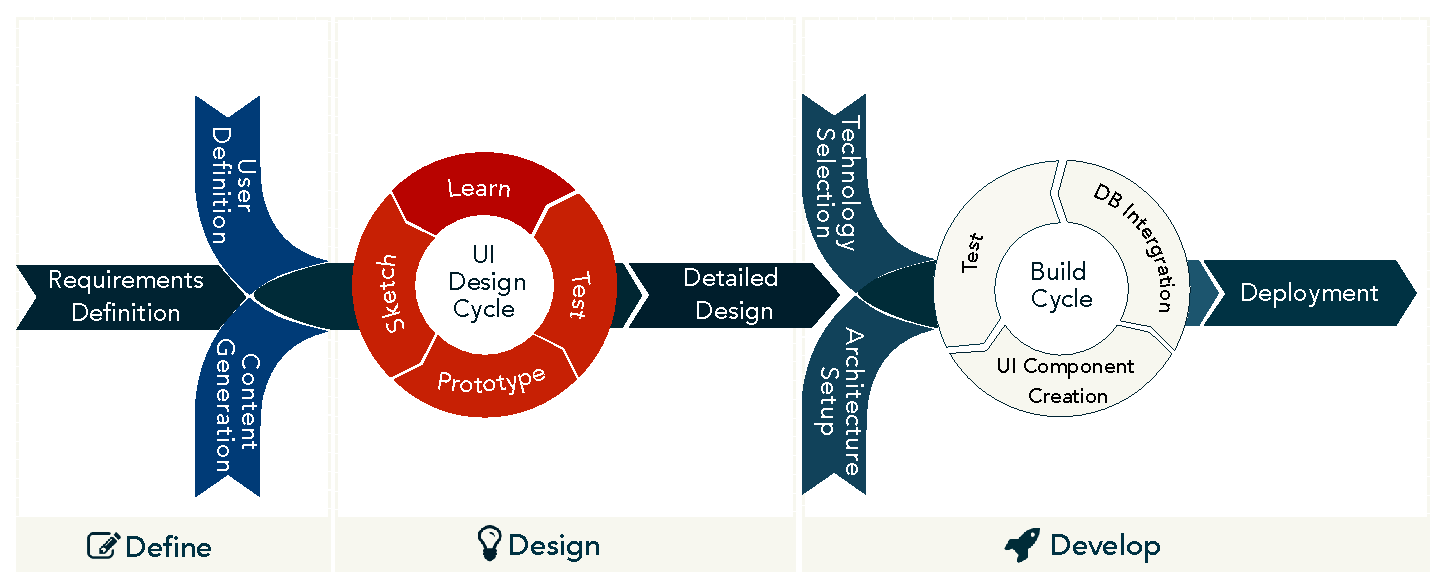
\includegraphics[trim = 0 0 0 0, clip, width=0.98\textwidth]{DesignProcess.eps}
\caption{Diagram illustrating the design process progressing the from the initial briefing to implementation}
\label{designprocess}
\end{figure}

\hypertarget{definition-phase}{%
\subsection{Definition Phase:}\label{definition-phase}}

This phase focused on collecting requirements and defining the
objectives of the project. In order to capture all the information
correctly, several meetings were held with the client these meetings
meetings were used to capture the main features of the site, creating
and organising the content that would be displayed. User research was
then embarked, refining the objectives and content of the site. These
stages all worked towards providing all the prior research required to
begin designing, prototyping and envisioning how the website would
function.

\hypertarget{design-phase}{%
\subsection{Design Phase:}\label{design-phase}}

The design phase applied human computer interaction (HCI) principles in
an agile to approach, to mock up variety of different solutions and
refine the solutions quickly. By following of the process of creating
sketches of different components of the website, whittling these
sketches down to wireframes and prototypes. Solutions could be quickly
tested by the designers, client and user groups providing feedback to
take back and learn upon, improving the overall design of the website
until a rough solution was generated which met both the design
objectives and the met HCI objectives. Spending time before writing any
code was key to making sure the solution was user friendly and visual
meeting one of the key objectives of the project. After rough solution
was created through user interface (UI) design cycle, this was then
padded out and refined creating a static draft of the design which could
be directly copied in the development phase. A large amount of time
could be saved in the development phase of the project by having a
finalised design template to work of which included the typography,
components and the page layouts of the site.

\hypertarget{development-phase}{%
\subsection{Development Phase:}\label{development-phase}}

Development was the final phase of the project. A complete understanding
of how the final product will look and function, based on the research
conducted in the definition phase and the detailed design template in
the design phase meant that all the technology required to required to
implement the solution can be selected. A local development environment
shared amongst all the developers enabled the use of an agile build
cycle, using git to mediate between the different versions. The build
cycle consisted of a developer taking a UI component from the template
and creating the design in code. This would then be connected to the PHP
database using word-press and the tested. Any bugs in either the design
or functionality could then be ironed out through iteration through the
cycle eventually integrating all the components together into the final
site. Once the entire design template was implemented the project could
then be deployed onto the web.

\newpage

\hypertarget{user-research}{%
\section{User Research}\label{user-research}}

this is some nice text bellow is an image.
\cite{blanchard2003macroeconomic}

\hypertarget{this-is-a-sub-heading}{%
\subsection{This is a sub heading}\label{this-is-a-sub-heading}}

\begin{figure}[H]
      \centering
      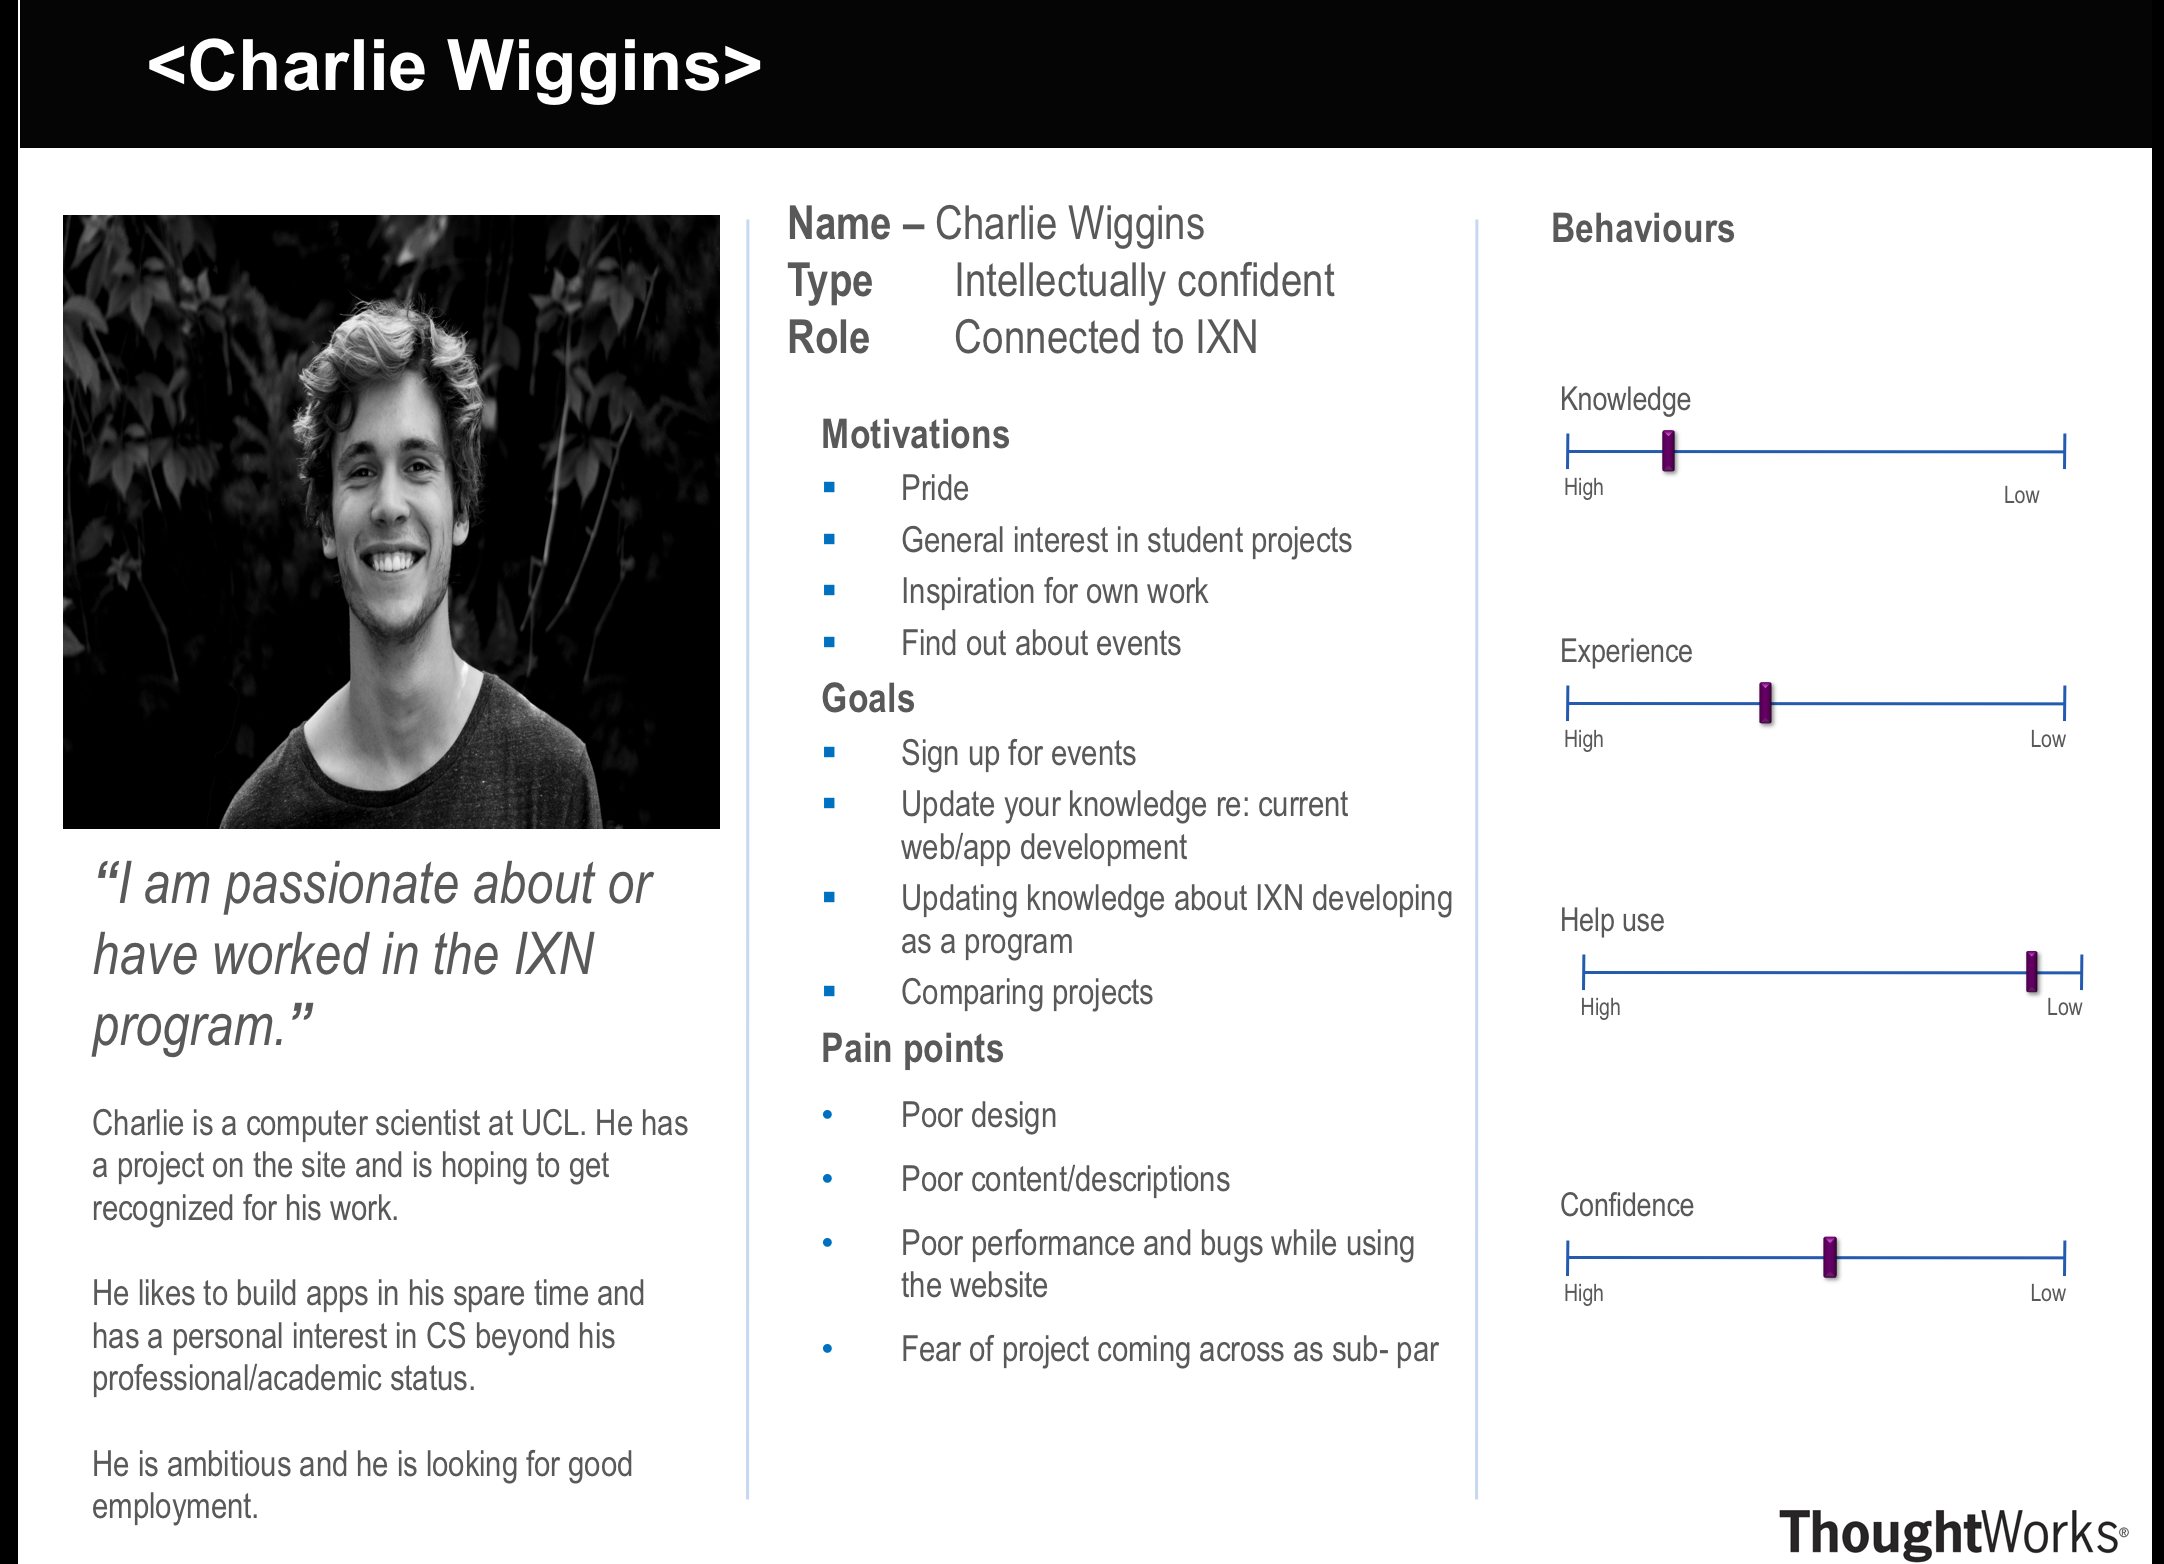
\includegraphics[trim = 0 0 0 0, clip, width=0.7\textwidth]{persona1.png}
      \caption{This is a persona}
      \label{persona1}
 \end{figure}

this image \cite{rumelt2012good} is of persona1 it is pretty good
\ref{persona1} \newpage

\hypertarget{technical-research}{%
\section{Technical Research}\label{technical-research}}

\newpage

\hypertarget{system-architecture}{%
\section{System Architecture}\label{system-architecture}}

In order to be able to create a high performance website, using the
latest technologies to optimises run time and speed up the design
process; a stack of Wordpress technologies were used in three tier
system architecture. The stack was run across both local and production
servers enabling a testing environment which was fully representative of
the production server while all code could be kept offline.

The full open source Roots stack \cite{rootsweb} was selected as it
provided all the tools and structure required to develop the project to
a professional standard. Figure \ref{systemarchitecture} shows the
relationship between the three roots technologies; Sage, Bedrock and
Trellis, and their relationship to the system architecture.

\begin{figure}[H]
\centering
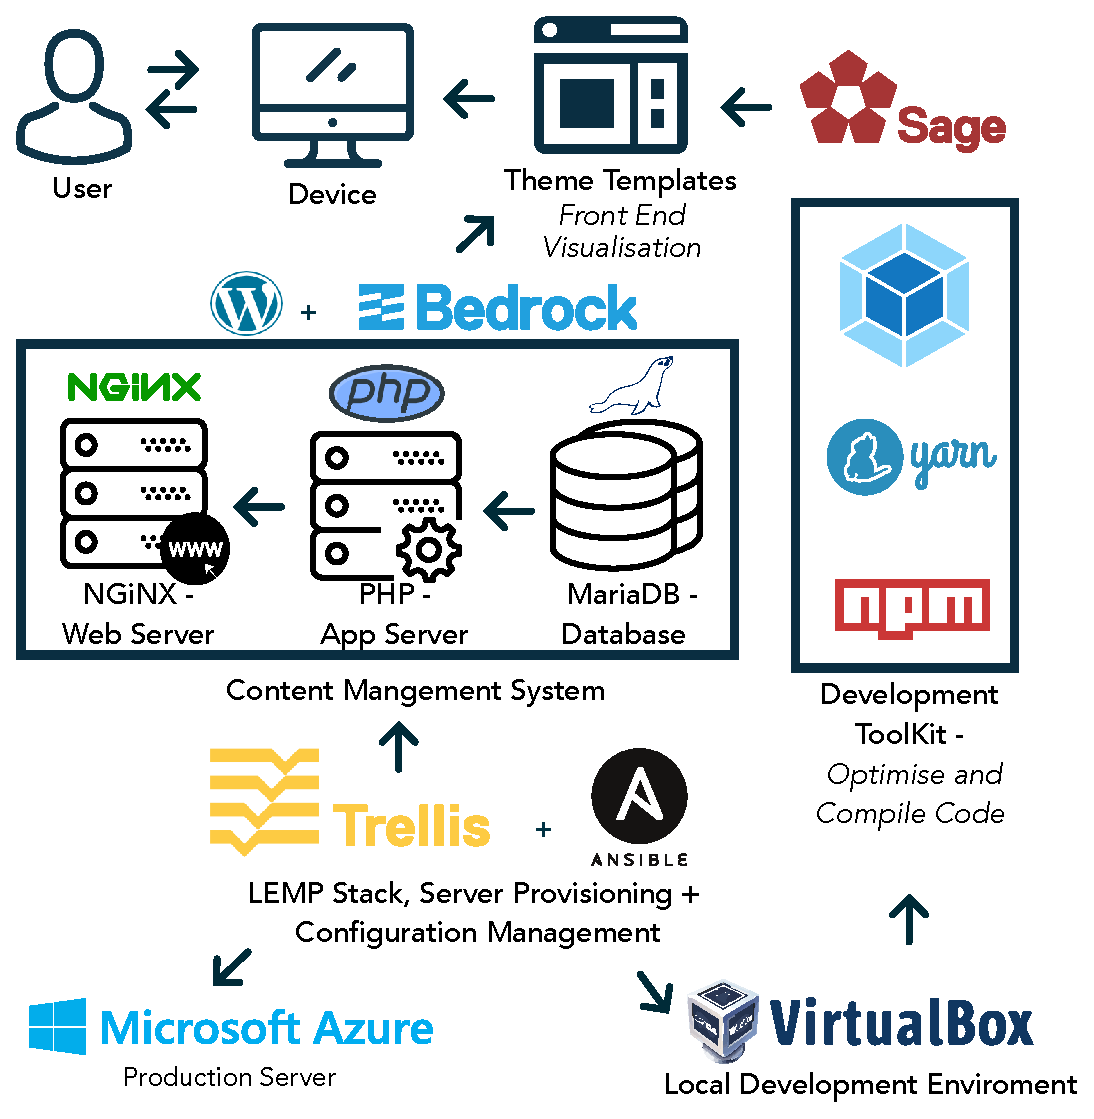
\includegraphics[trim = 0 0 0 0, clip, width=0.85\textwidth]{SystemArchitecture.eps}
\caption{Diagram showing the websites systems architecture, highlighting the relationship between different technologies}
\label{systemarchitecture}
\end{figure}

\newpage

\hypertarget{implementation}{%
\section{Implementation}\label{implementation}}

\hypertarget{testing}{%
\section{Testing}\label{testing}}

\newpage

\hypertarget{conclusion}{%
\section{Conclusion}\label{conclusion}}

\newpage
% -----------------------------------------------------------------------------------
%                                  APENDIX
% -----------------------------------------------------------------------------------

% \end{counted} %<<<<<<<<<<<<<<ENDS WORD COUNTER

\newpage
% \section{Appendices}
% Above were \thewords\ words. %<<<<<<<<<<<<<<DISPLAYS WORD COUNTER
% -----------------------------------------------------------------------------------
%                               BIBLIOGRAPHY - Insert Name of BIB File Here
% -----------------------------------------------------------------------------------
\newpage

% ---------------BIBTEX OLD-----------------------------------------------------
% \bibliographystyle{unsrt} %%%% Plain or alpha can change orders here
% \bibliography{BibFile}
% \nocite{*} %%%if you want to see all references even those note cited in the text
% -----------------------------------------------------------------------------------

\printbibliography

\end{document}
